% !TEX encoding = UTF-8
%Koma article
\documentclass[fontsize=12pt,paper=letter,twoside]{scrartcl}
\usepackage{float}
\usepackage{url}

%Standard Pre-amble
\usepackage[top=4cm,bottom=4cm,left=3cm,right=3cm,asymmetric]{geometry}
%\geometry{landscape}                % Activate for for rotated page geometry
%\usepackage[parfill]{parskip}    % Begin paragraphs with an empty line rather than an indent
\usepackage[table,xcdraw]{xcolor}
\usepackage{graphicx}

\usepackage{amsmath}
\usepackage{amssymb}
\usepackage{epstopdf}
\DeclareGraphicsRule{.tif}{png}{.png}{`convert #1 `dirname #1`/`basename #1 .tif`.png}
% Listings needs package courier
\usepackage{listings} % Needs 
\usepackage{courier}

\usepackage[framemethod=TikZ]{mdframed}
\usepackage{url}

\usepackage{sty/bsymb} %% Event-B symbols
\usepackage{sty/eventB} %% REQ and ENV
\usepackage{sty/calculation}

%Maths
\usepackage{amssymb,amsmath}
\def\Fl{\mathbb{F}}
\def\Rl{\mathbb{R}}
\def\Nl{\mathbb{N}}
\def\Bl{\mathbb{B}}
\def\St{\mathbb{S}}
\newcommand{\ovr}{\upharpoonright}
\newcommand{\var}[1]{\textit{#1}}
%Useful definitions
\newcommand{\mv}[1]{\textit{m\_#1}}
\newcommand{\cv}[1]{\textit{c\_#1}}
\newcommand{\degree}[1]{^{\circ}\mathrm{#1}}
%\newcommand{\comment}[1]{{\footnotesize \quad\texttt{--}\textrm{#1}}}
\newcommand{\im}[1]{i\texttt{-\!#1}}

\usepackage[headsepline]{scrpage2}
\pagestyle{scrheadings}
\ihead[]{\small EECS4312 Report1}
\ohead[]{\small \thepage}
\cfoot[]{}
\ofoot[]{}


%%%%PVS environment%%%%%%%%%%%%%%%%%%%
\lstnewenvironment{pvs}[1][]
    {\lstset{#1,captionpos=b,language=pvs,
    mathescape=true,
    basicstyle=\small\ttfamily,
    numbers=none,
    frame=single,
    % numberstyle=\tiny\color{gray},
    % backgroundcolor=\color{lightgray},
    firstnumber=auto
    }}
    {}
 %%%%%%%%%%%%%%%%%%%%%%%%%%%%%%%%
 
%%%%Verbatim environment%%%%%%%%%%%%%%%%%%%
\lstnewenvironment{code}[1][]
    {\lstset{#1,captionpos=b,
    mathescape=true,
    basicstyle=\small\ttfamily,
    numbers=none,
    frame=single,
    % numberstyle=\tiny\color{gray},
    % backgroundcolor=\color{lightgray},
    firstnumber=auto
    }}
    {}

% \newenvironment{boxed}[1]
%    {\begin{center}
%    #1\\[1ex]
%    \begin{tabular}{|p{0.9\textwidth}|}
%    \hline\\
%    }
%    { 
%    \\\\\hline
%    \end{tabular} 
%    \end{center}
%    }
 %%%%%%%%%%%%%%%%%%%%%%%%%%%%%%%%
 
 %Text in a box
\newenvironment{textbox}
    {\begin{center}
    \begin{tabular}{|p{0.9\textwidth}|}
    \hline\\
    }
    { 
    \\\\\hline
    \end{tabular} 
    \end{center}
    }

\usepackage{hyperref}

%Highlight \hl{}
\usepackage{soul}

\usepackage{enumitem}
\newlist{mylist}{itemize}{1}
\setlist[mylist]{label=\textbullet,leftmargin=1cm,nosep}

\usepackage{multirow}

% Reduce space between figure and caption
%\usepackage{caption}
%\captionsetup[table]{font=small,skip=0pt}     %% Adjust here
%or equivalently 
\usepackage[font=small,skip=4pt]{caption}
%Useful definitions
%\newcommand{\mv}[1]{\textit{m\_#1}}
%\newcommand{\cv}[1]{\textit{c\_#1}}
%\newcommand{\degree}[1]{^{\circ}\mathrm{#1}}
%\newcommand{\comment}[1]{{\footnotesize \quad\texttt{--}\textrm{#1}}}

% Set the header
\ihead[]{\small EECS4090 Project}


%%%%%%%%%%%%Enter your names here%%%%%%%%
\author{\textbf{Edward Vaisman}
\and \textbf{Sadman Sakib Hasan}
}
%%%%%%%%%%%%%%%%%%%%%%%%%%%%%%%%

\date{\today} % Display a given date or no date

\begin{document}
\title{Grad Apps 2.0 Design Documentation}
\maketitle

\newpage

\section*{Revisions}

%%%%%%%%%%%%Table of revisions%%%%%%%%
\begin{tabular}{|l|l|p{3in}|}
\hline
Date & Revision & Description \\ 
\hline
22 November, 2017
& 1.0
& Initial Document Draft \\
\hline
4 December, 2017
& 1.1
& Included UML Class Diagram and Rationale \\
\hline
12 December, 2017
& 1.2
& Updated the Class diagram (Model section Role separation), Added Entity-Model Diagram, Added Data descriptions \\
\hline
14 December, 2017
& 1.3
& Updated Class diagram to match the new model, Updated Entity-Model Diagram, Edited Data descriptions \\
\hline
16 December, 2017
& 1.4
& Added Interface Design and Traceability Matrix \\
\hline
17 December, 2017
& 1.5
& Added Sequence Diagrams for the Component Design \\
\hline
19 January, 2018
& 1.6
& Updated Data Dictionary and Model Diagram \\
\hline
\end{tabular}
%%%%%%%%%%%%%%%%%%%%%%%%%%%%%%%%

\newpage

%%%%%%%%%%%%%%%%%%%%%%%%%%%%%%%
\tableofcontents
\listoffigures
\listoftables
\newpage


%%%%Rest of your document goes here%%%%%%%%%%%%%%%%%%%

\clearpage
\section{Introduction}

\subsection{Purpose}

This software design document is intended to provide information regarding the system and architecture on the design of the new graduate application system for the EECS graduate program.

\subsection{Scope}

Gradapps v2.0, a graduate application system, is intended to assist the EECS graduate program better locate and maintain potential graduate student applications from the moment it is submitted until the moment a decision is made. It is intended to replace the current system in use for the EECS graduate program. It will be accessible for use as an online portal on the web.

\smallskip
\noindent Gradapps v2.0 promises the following:
\begin{itemize}
\item \emph{Administrators} will be able to manage \emph{Committee Members}, assign applications to \emph{Committee Members} to review, edit/manage student applications, grant/revoke privileges from faculty members and add/remove members from the system.
\item \emph{Committee Members} will be able to view and manage a list of student applications assigned to them and be able to save applications as a draft for future edits.
\item \emph{Professors} will be able to search for applications and indicate their interest in a student to other professors and for personal use indicate whether or not an application has been reviewed.
\item All roles will be able to apply advanced filtering methods relative to their given roles to help search for applications.
\end{itemize}

\newpage
\subsection{Overview}

This document is divided into 9 sections,

\begin{itemize}
\item Introduction
\item System Overview
\item System Architecture
\item Data Design
\item Component Design
\item Human Interface Design
\item Requirement Matrix
\item Appendices
\end{itemize}

%%%%%%%%%%%%%%%%%%%%%%%%%%%%%%%%%%%%%%%%%%%

\newpage
\section{System Overview}

Having a postgraduate degree on one's resume is always appealing to their future employer, let it be working in the industry or continuing studies to achieve a doctoral status. When applying for a postgraduate program, applicants spend a lot of their time gathering different levels of information (transcripts, letter of recommendation, resume etc.) required for admission. Once an application has been submitted, the graduate program analyses the information to find the best candidate for each program.

\smallskip
Analysing that level of dense information can be challenging at times and to avoid loss of any information, it is best practice to automate this process as much as possible. In order to achieve that goal, a \emph{concise} and \emph{simple} Business System is required that will reduce the manual work.

\smallskip
The graduate program in Electrical Engineering and Computer Science (EECS) is facing a very similar situation. The current system our client has involves a lot of manual work. The centre of this process are the Graduate Program Director (GPD) and Graduate Program Assistant (GPA) who plays a major role in all applications regardless of the applicant being admitted or rejected.

\smallskip
\emph{Administrators} have the task of managing \emph{Committee Members}, acquiring documents from the admissions office for upload, assigning applications to \emph{Committee Members} for review, assigning roles to faculty members, uploading applications for faculty members to view, and lastly manage student applications.

\smallskip
\emph{Committee Members} have the task of reviewing an application provided by the Administrator(s) and send it back for the \emph{Administrators} to upload once all reviews are in for Faculty Members to see.

\smallskip
\emph{Professors} then have the ability to search for applications that best suit their criteria for a good graduate student.

\smallskip
Given the current restrictions with York admissions office some things such as accessing different levels of information must be done manually by the \emph{GPA} other types of accessing information such as, looking up a university description could be done automatically. Overall, our client requires a more robust and concise system that will enable them to automate the selection of the best candidate into the program minimizing the manual work.

%%%%%%%%%%%%%%%%%%%%%%%%%%%%%%%%%%%%%%%%%%%

\newpage

\section{System Architecture} \label{sec:system_architecture}
\subsection{Architectural Design}
\begin{figure}[!htb]
\begin{center}
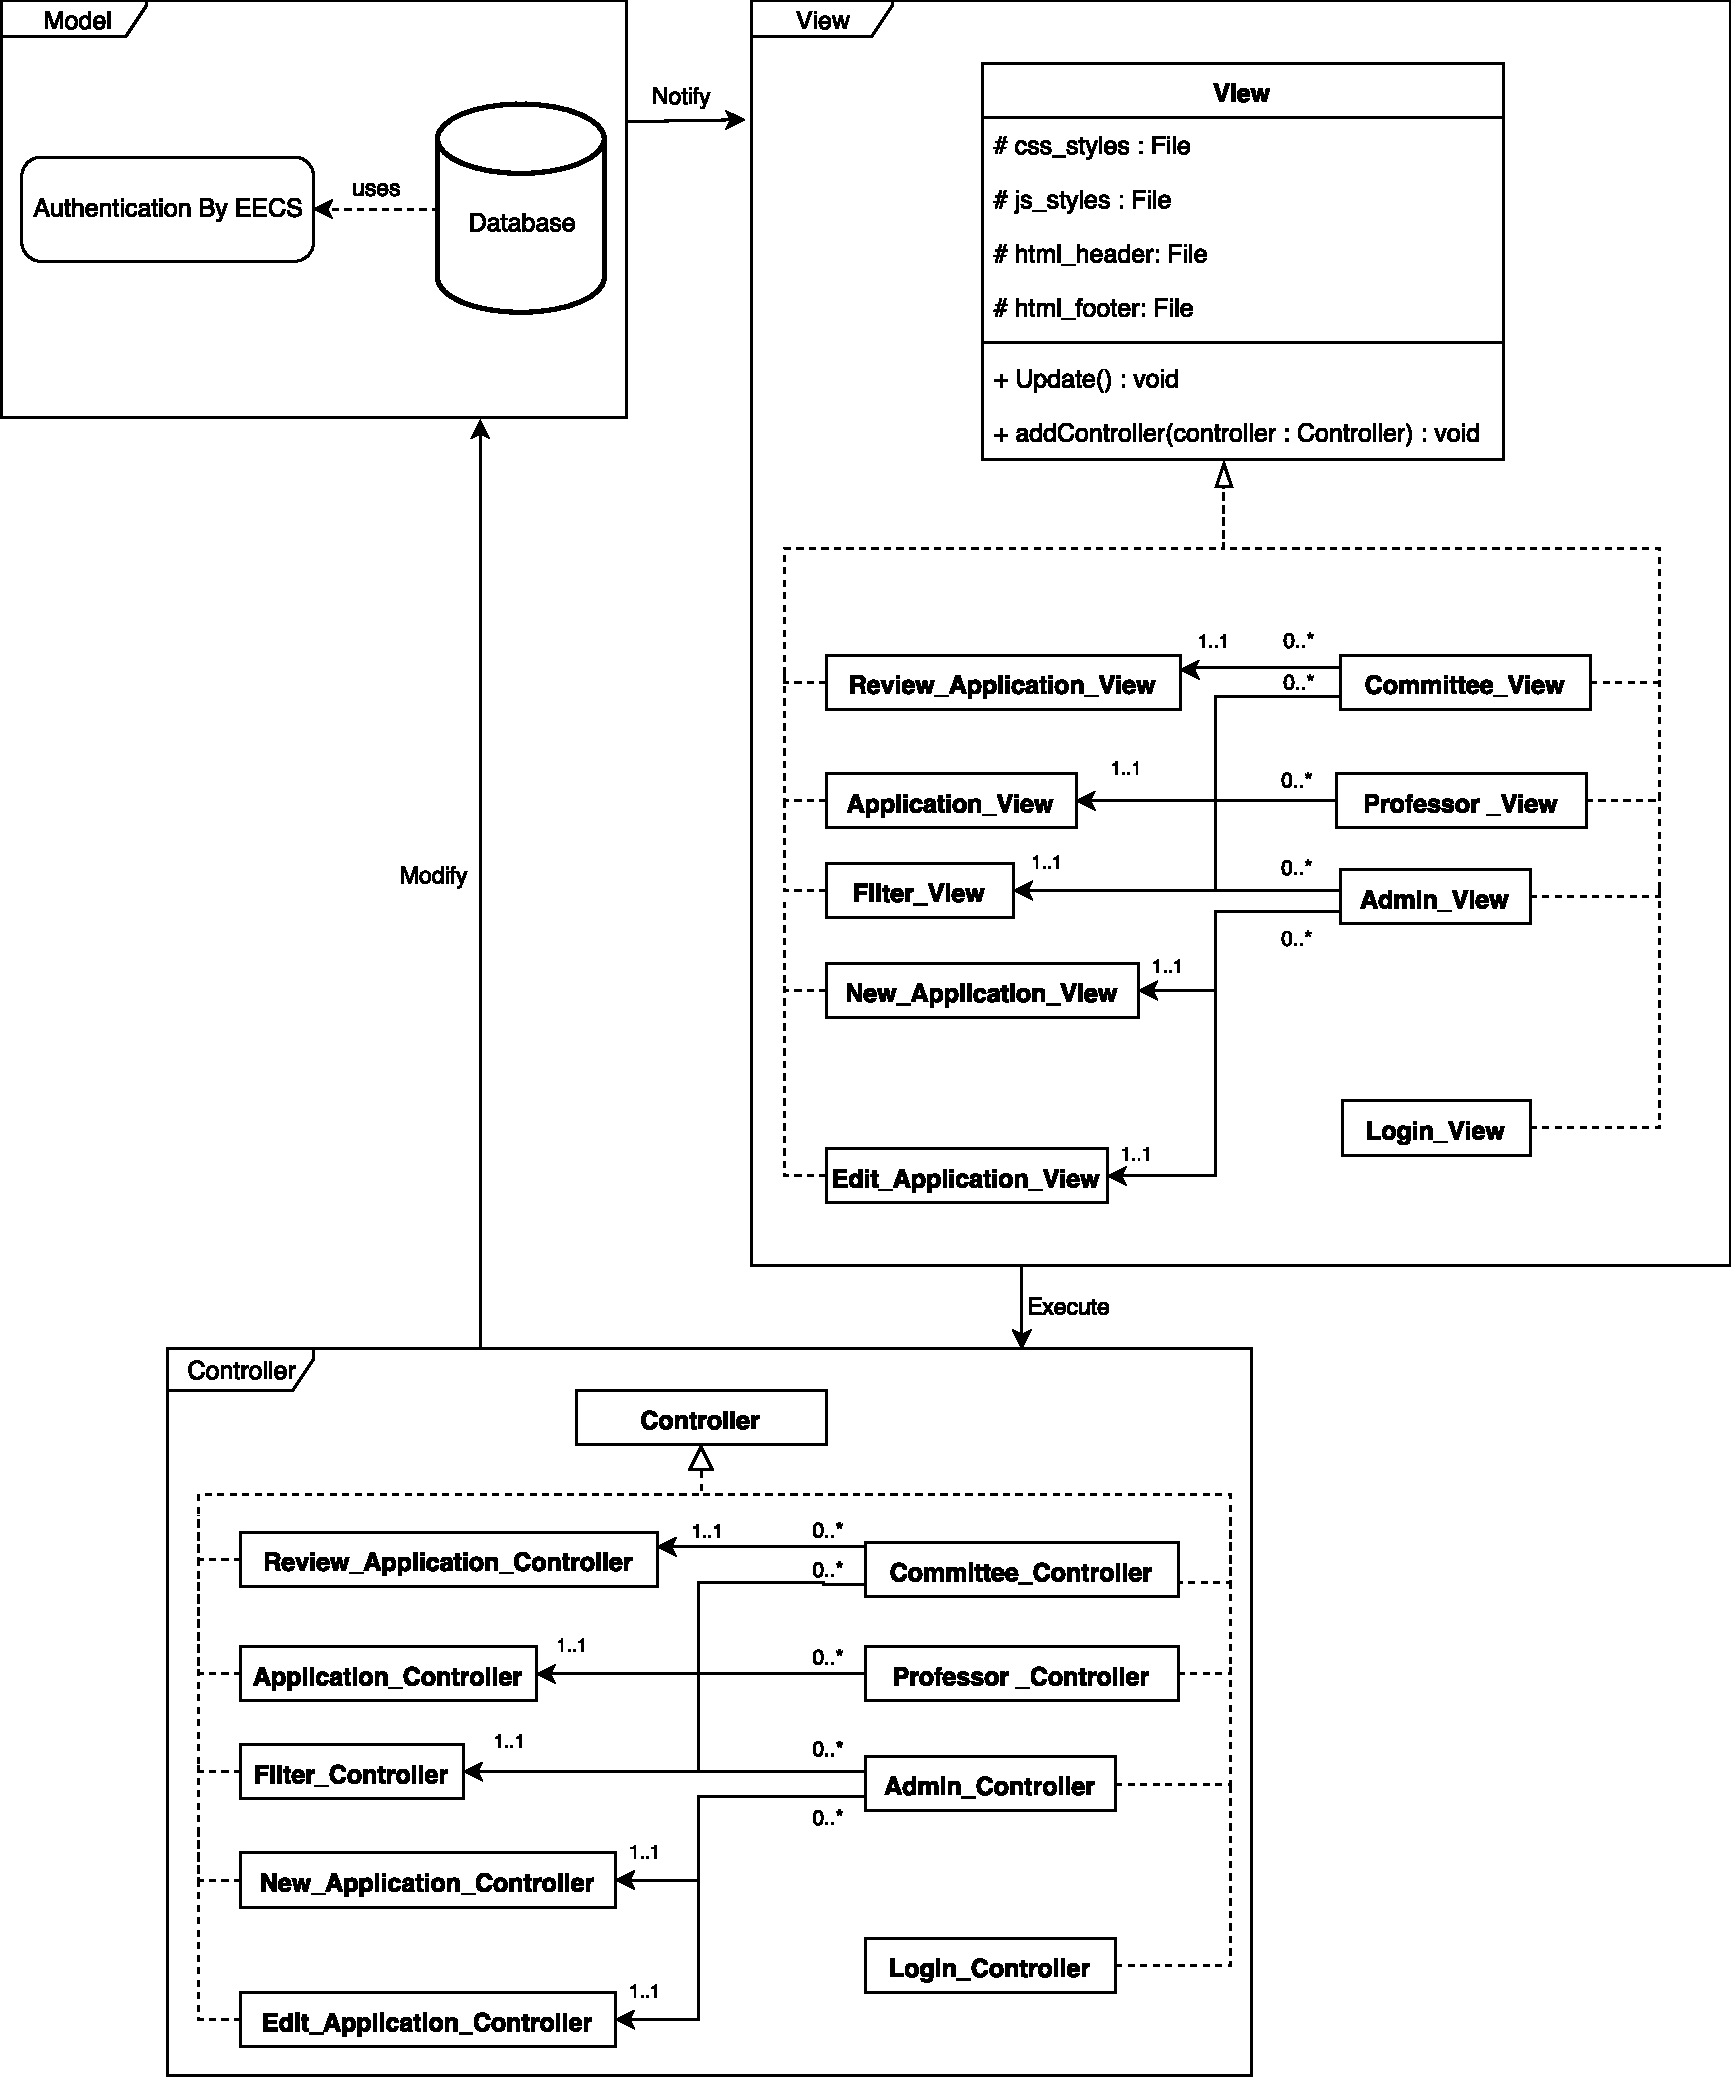
\includegraphics[width=.85\textwidth]{images/class_diagram.pdf}
\end{center}
\caption{UML Class Diagram}
\label{fig:uml_class_diagram}
\end{figure}

\newpage
\subsection{Decomposition Description}

The System Architecture was designed with the MVC Pattern in mind.

\begin{itemize}
\item The \emph{Model} represents the database and acts as a data handler for all the data to be stored.

\item The \emph{View} represents the front-end web application using web technologies such as html, css and javascript. 

\item The \emph{Controller} represents the back-end system that triggers the model and updates the view.
\end{itemize}


\subsection{Design Rationale}

\subsubsection{MVC}

Given that this is a web application designing it using the MVC pattern makes the most sense here for the following reason:

\begin{itemize}
\item Simultaneous development
\item Ease of modification
\item Multiple Views for our one model
\end{itemize}

As a result of MVC, developers will be able to work on parts of the system concurrently as opposed to having to wait for others to finish their part and the ability to add or remove a feature later on will be easier and the overall system will be modular.

\subsubsection{Roles}

To satisfy the specification requirements of faculty members being able to have more than one role, there is no inheritance/generalization between  faculty members and all the other roles. This design choice allows for an easy separation of information across roles so that changes in one does not affect changes in another.

An alternative to this design would have been to split the roles into their own classes. This choice is not beneficial for our system since all of our roles share common things such as id, name, email etc… and would create a lot of duplication in the system. See Section \ref{sec:data_design} for diagram and data description.

%%%%%%%%%%%%%%%%%%%%%%%%%%%%%%%%%%%%%%%%%%%

\newpage
\begin{figure}[!htb]
\section{Data Design} \label{sec:data_design}
\subsection{Data Description}

The following diagram illustrates the UML Entity Relationship. The design of each entity will be represented in the database during the implementation phase.
\begin{center}
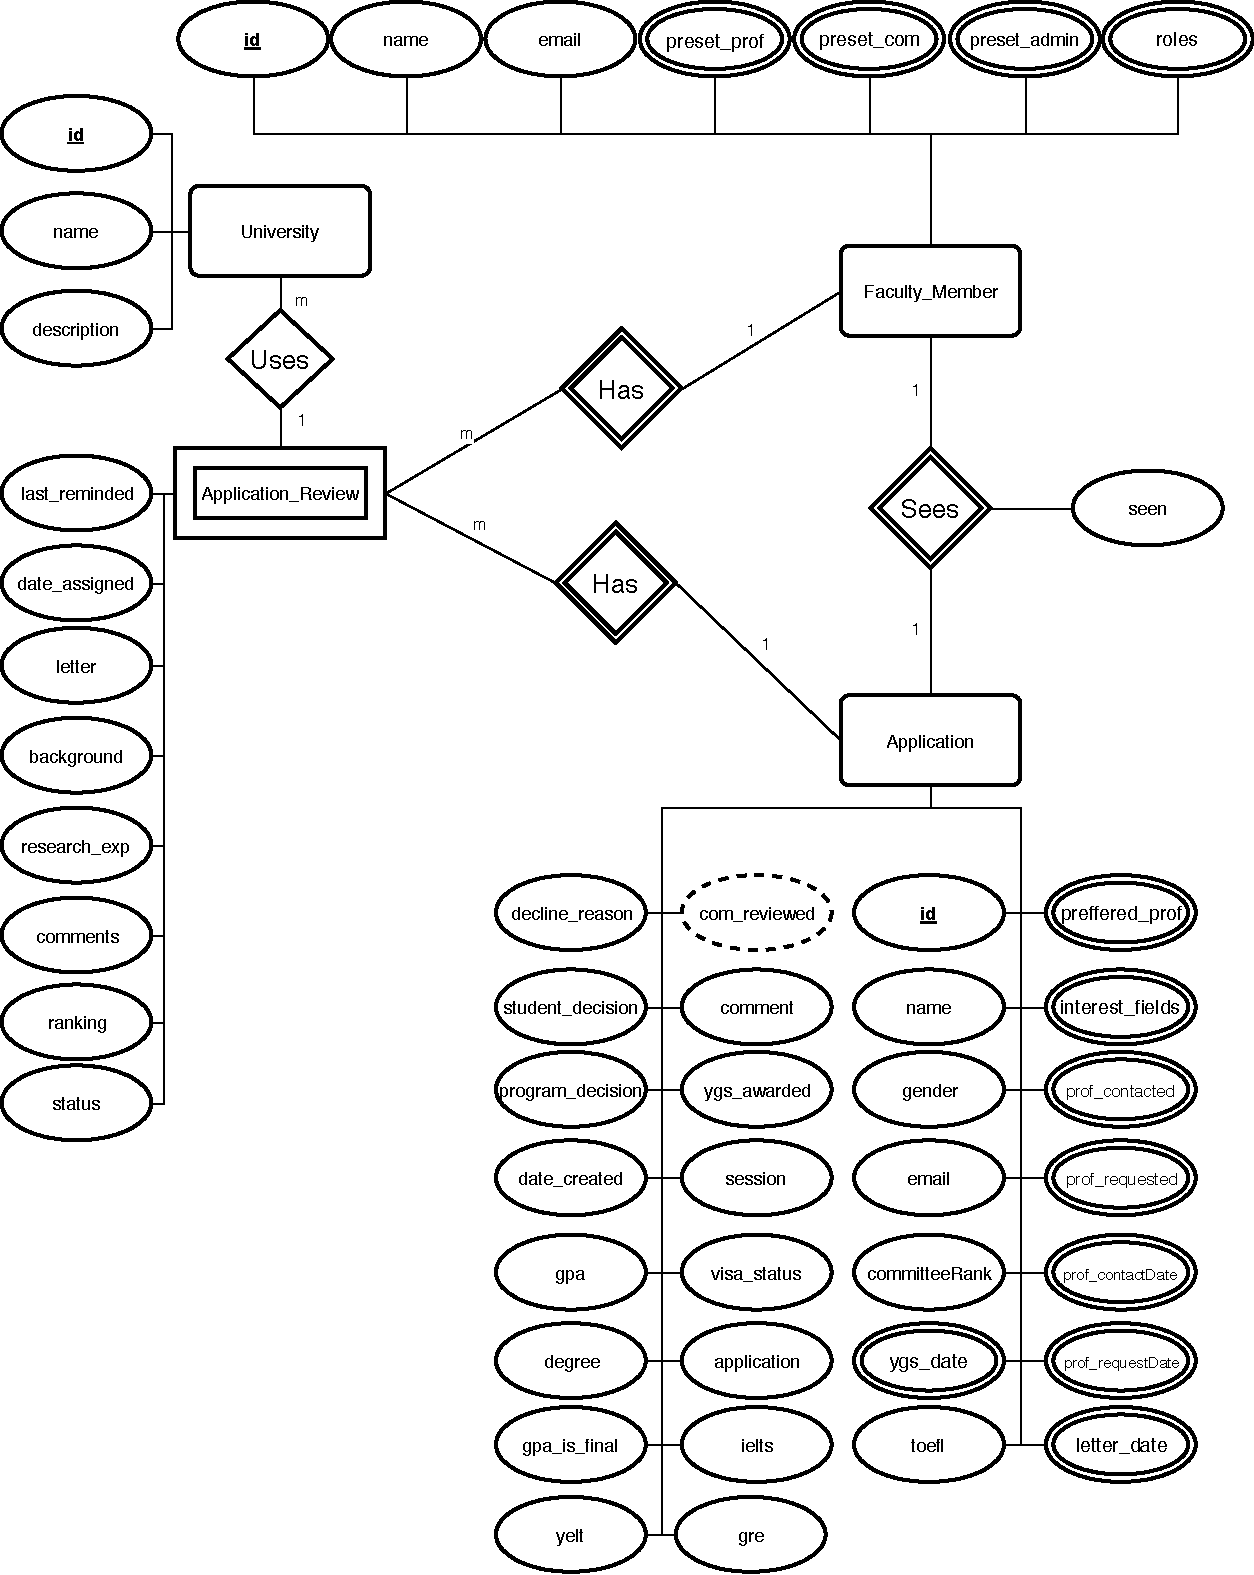
\includegraphics[width=.99\textwidth]{images/entity_relation.pdf}
\end{center}
\caption{Entity Relation Diagram}
\label{fig:uml_entity_diagram}
\end{figure}


\clearpage
\newpage

\begin{figure}[!htb]
\subsection{Data Dictionary}
\begin{center}
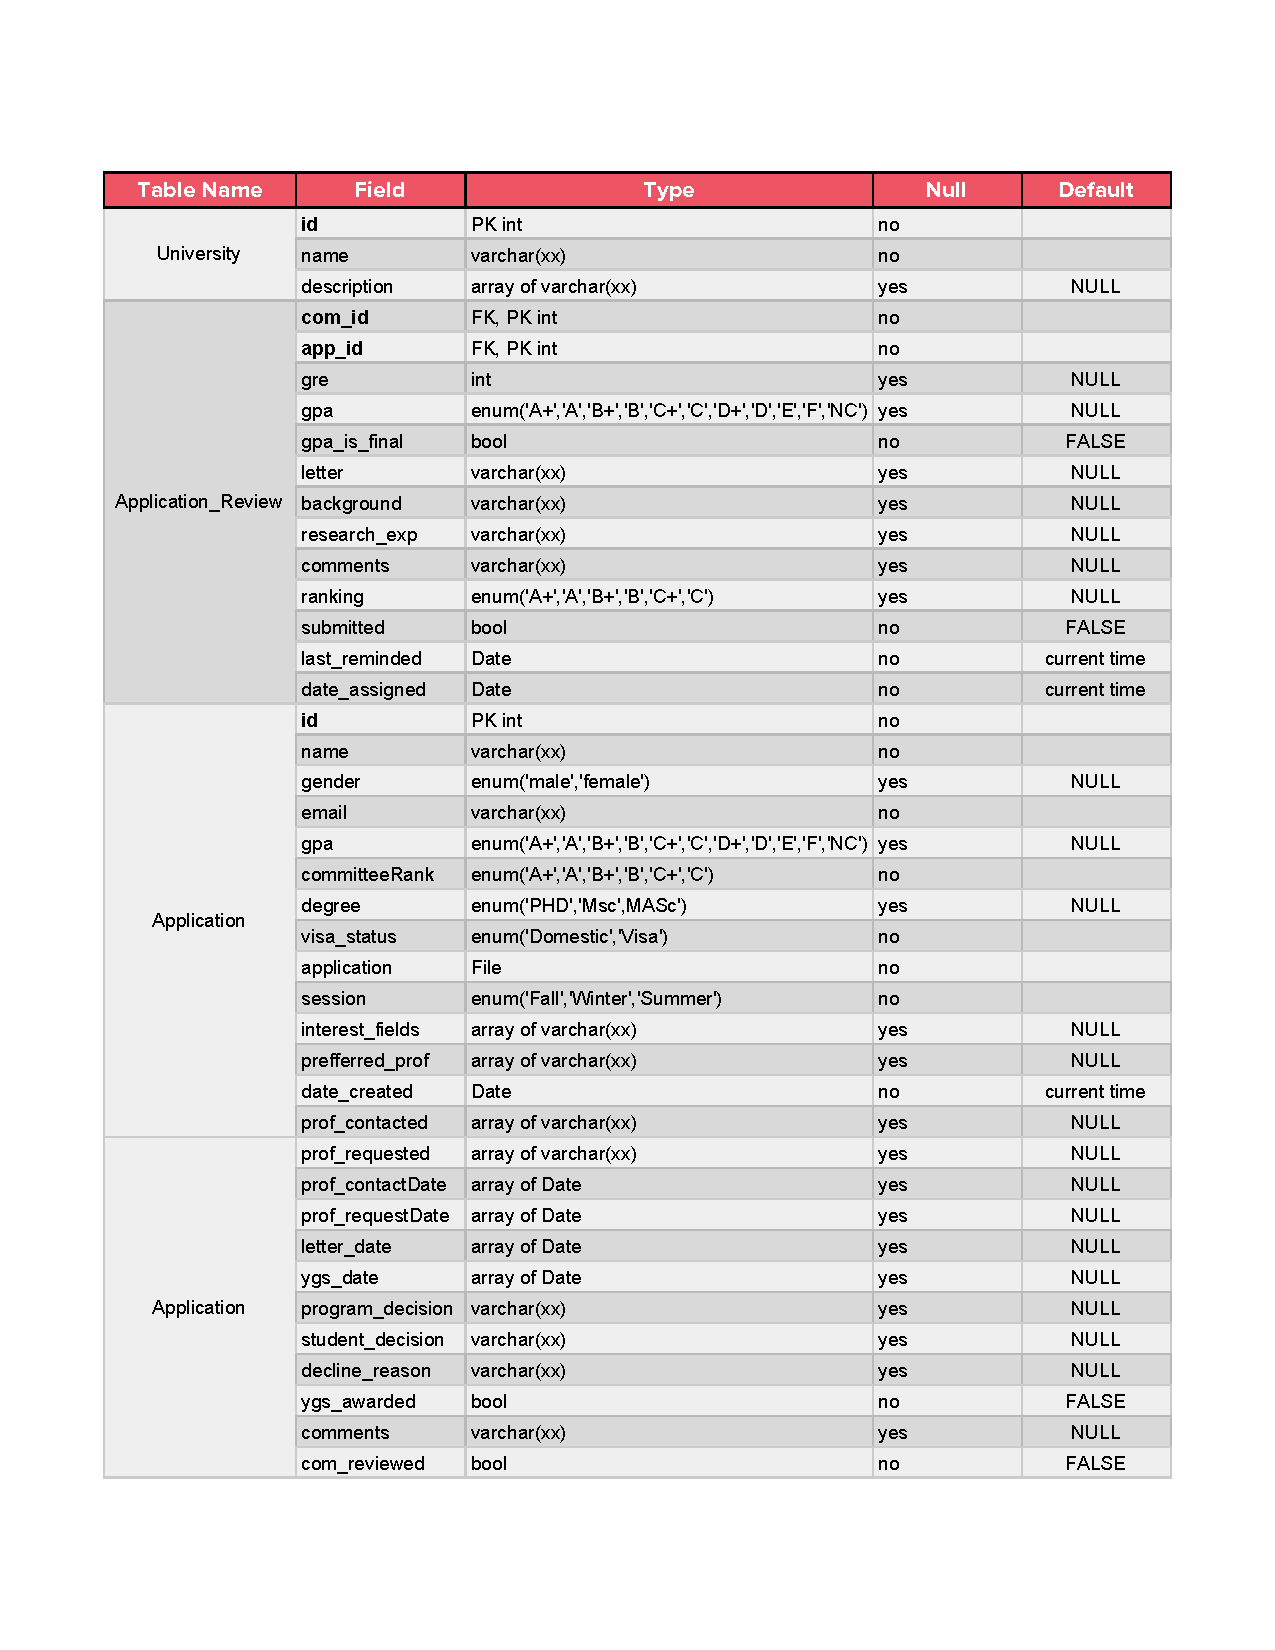
\includegraphics[width=\textwidth]{images/data_dictionary1.pdf}
\end{center}
\caption{Data Dictionary Part.1}
\label{fig:dd1}
\end{figure}

\clearpage
\newpage

\begin{figure}[!htb]
\begin{center}
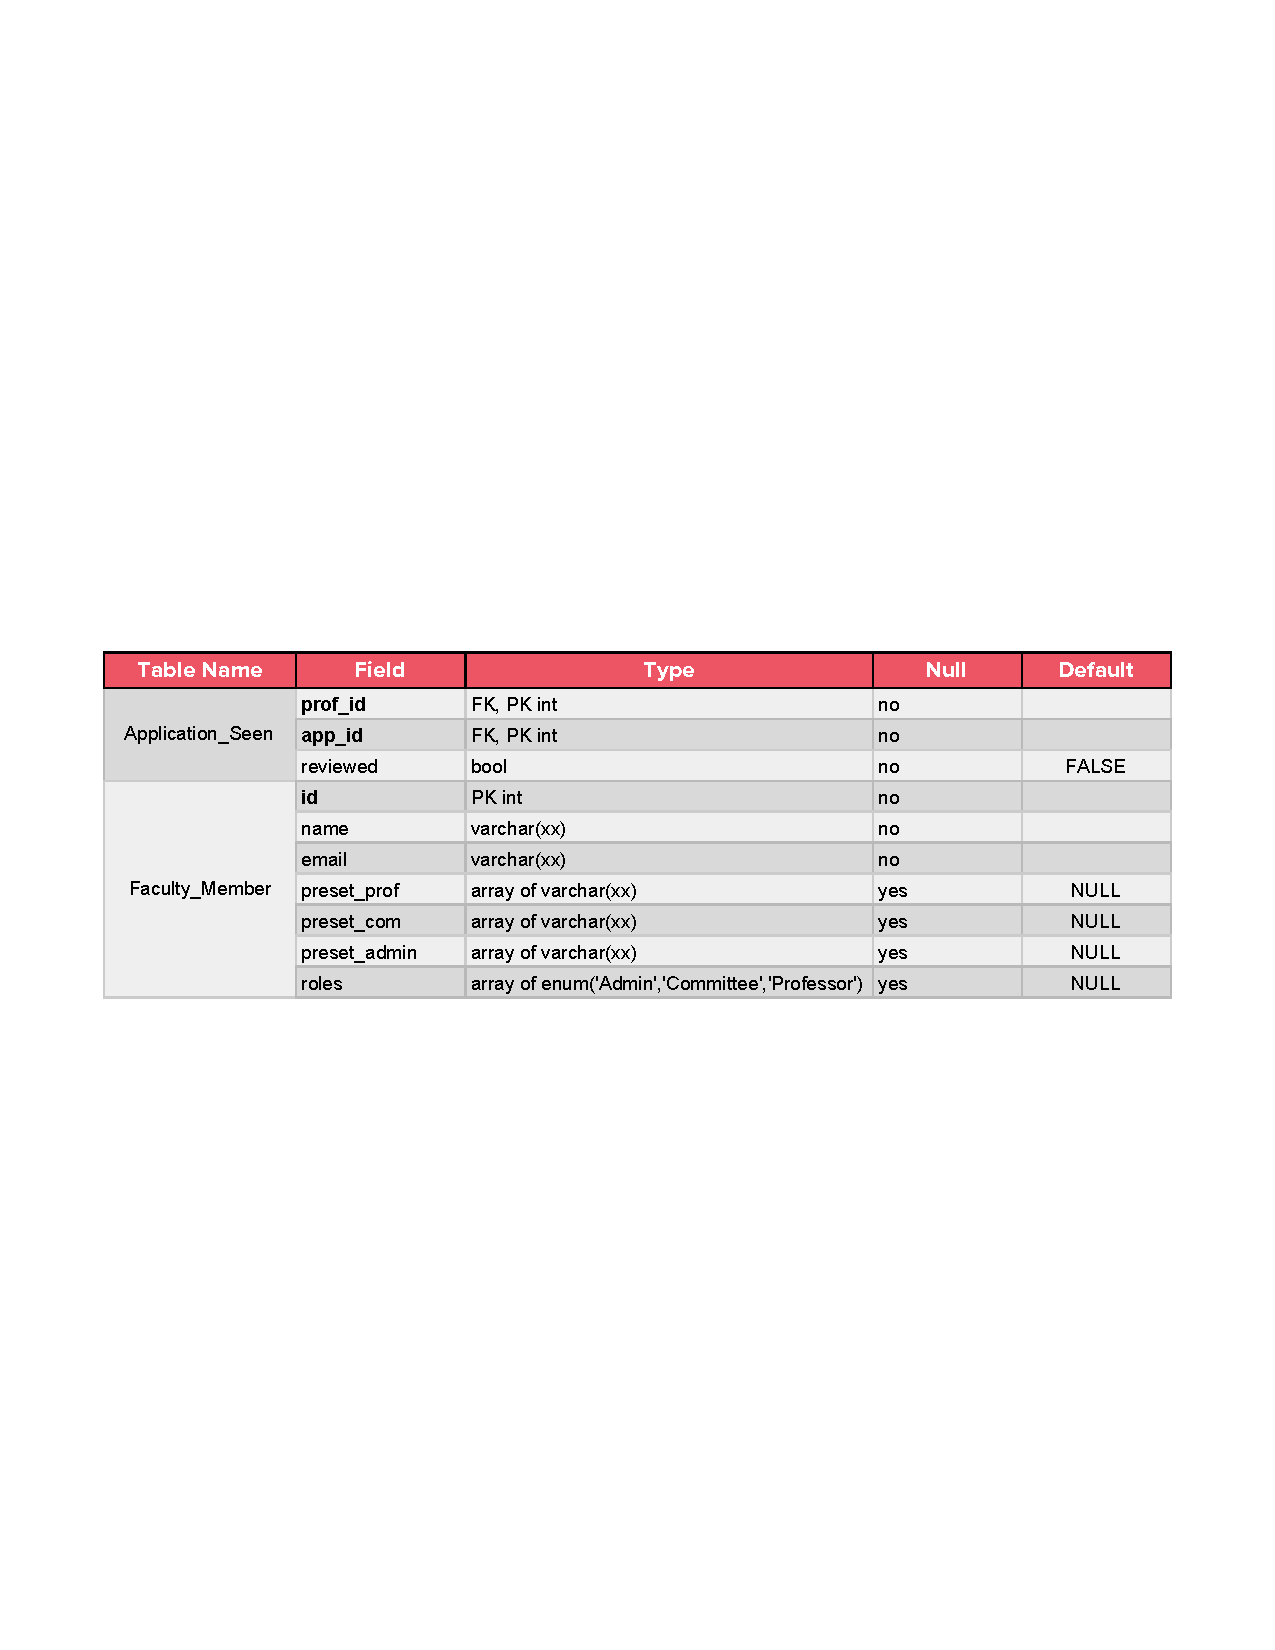
\includegraphics[width=\textwidth]{images/data_dictionary2.pdf}
\end{center}
\caption{Data Dictionary Part.2}
\label{fig:dd2}
\end{figure}

%%%%%%%%%%%%%%%%%%%%%%%%%%%%%%%%%%%%%%%%%%%

\clearpage
\newpage
\section{Component Design}

\subsection{Model}

The model acts as a data storage handler for the GradApps business system. Most of which is already discussed in Section \ref{sec:data_design}. The database will use MySQL version: 5.7.20 and Authentication By EECS as per the requirements elicited from the client. The design chosen was in favor of simplicity instead of efficiency. This decision was based on the relatively low amount of student applications gradapps will store (roughly 1000 applications per year) thus eliminating the need for faster query calls.

\subsection{View}
Some views will be able to display other views depending on the role selected.

\smallskip 
\noindent Here are a few:

\begin{itemize}
\item Admin View includes the Filter View, New Application View, Edit Application View,  and the Application View.
\item Committee View includes the Filter View, and the Review Application View.
\item Professor View includes the Application View, and the Filter View.
\end{itemize}

\noindent Based on what the main view is (Admin, Committee, Professor) the filter view will adjust accordingly to allow for their respective controllers.


\subsection{Controller}

Since some roles have different privileges than others, it is important to restrict what one user could do based on the view that they are in. For example, if someone is in the professor view they cannot access methods from the admin controller.

\subsubsection{Sequence Diagrams}

The following sequence diagrams describe the communication between our actors and the system under description. In short our system behaves as follows.

\begin{itemize}
\item Actor acts on the system
\item Client side validation
\item Appropriate updates to database
\item Return updated results and error message if necessary.
\end{itemize}

\begin{figure}[!htb]
\begin{center}
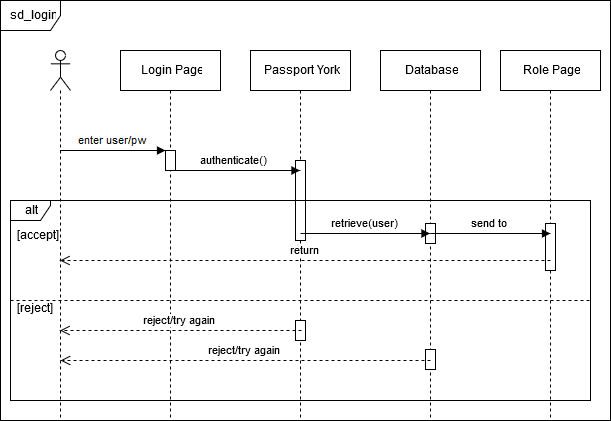
\includegraphics[width=.99\textwidth]{images/sd_login.png}
\end{center}
\caption{Sequence Diagram: Login to the system}
\label{fig:sd_login}
\end{figure}

\begin{figure}[!htb]
\begin{center}
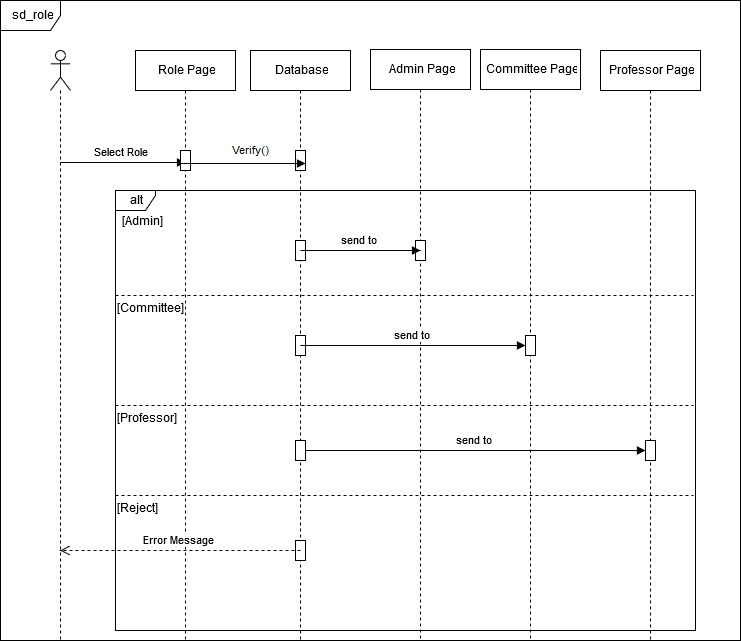
\includegraphics[width=.99\textwidth]{images/sd_role.png}
\end{center}
\caption{Sequence Diagram: Role Selection}
\label{fig:sd_role_selection}
\end{figure}

\begin{figure}[!htb]
\begin{center}
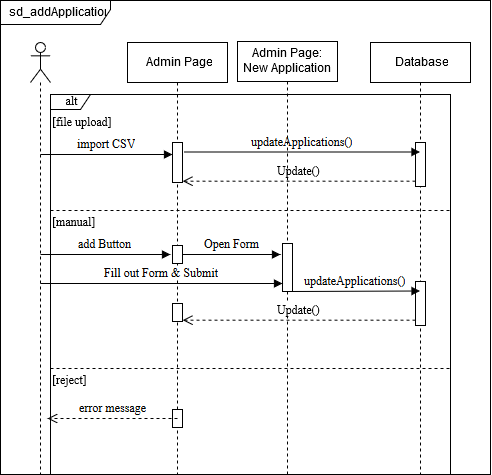
\includegraphics[width=.99\textwidth]{images/sd_addApplication.png}
\end{center}
\caption{Sequence Diagram: Upload an Application}
\label{fig:sd_add_application}
\end{figure}

\begin{figure}[!htb]
\begin{center}
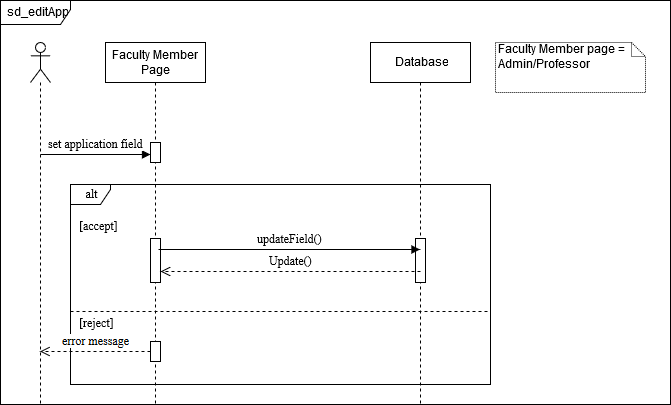
\includegraphics[width=.99\textwidth]{images/sd_editApp.png}
\end{center}
\caption{Sequence Diagram: Update an Application}
\label{fig:sd_update_application}
\end{figure}

\begin{figure}[!htb]
\begin{center}
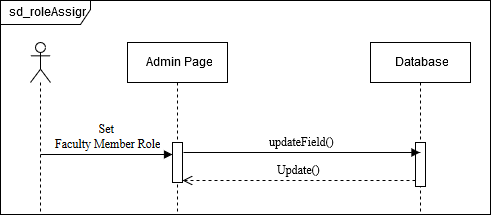
\includegraphics[width=.99\textwidth]{images/sd_roleAssign.png}
\end{center}
\caption{Sequence Diagram: Assigning a Role}
\label{fig:sd_assign_role}
\end{figure}

\begin{figure}[!htb]
\begin{center}
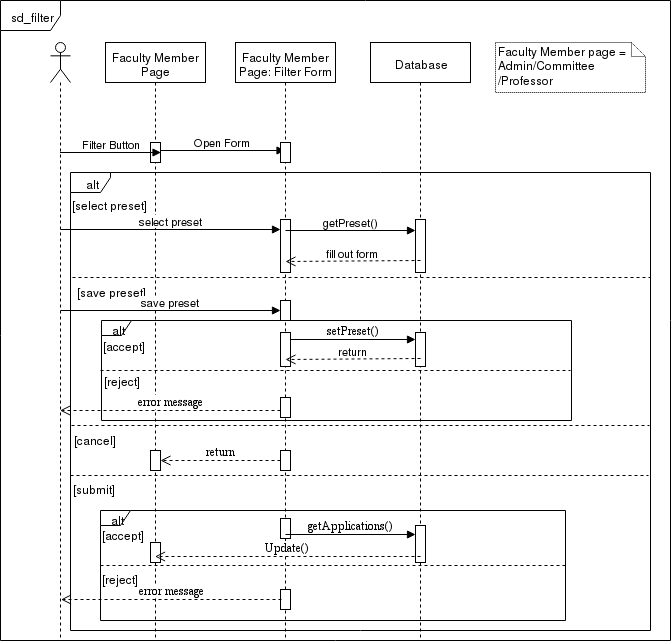
\includegraphics[width=.99\textwidth]{images/sd_filter.png}
\end{center}
\caption{Sequence Diagram: Applying filter}
\label{fig:sd_apply_filter}
\end{figure}

\begin{figure}[!htb]
\begin{center}
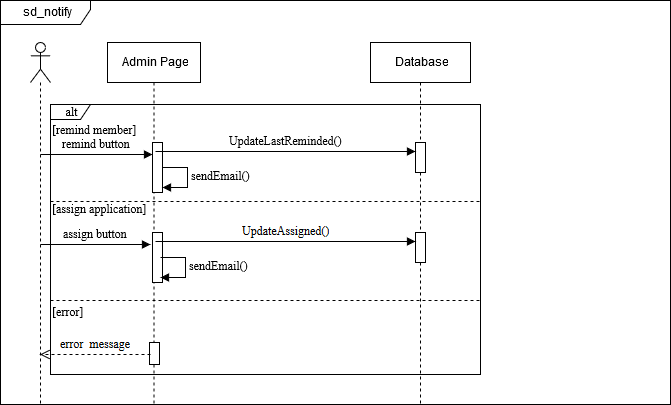
\includegraphics[width=.99\textwidth]{images/sd_notify.png}
\end{center}
\caption{Sequence Diagram: Notification}
\label{fig:sd_notification}
\end{figure}

\begin{figure}[!htb]
\begin{center}
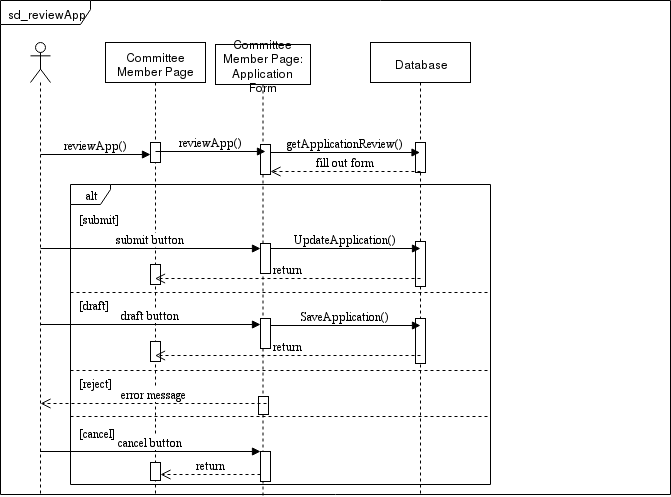
\includegraphics[width=.99\textwidth]{images/sd_reviewApp.png}
\end{center}
\caption{Sequence Diagram: Review an Application}
\label{fig:sd_review_application}
\end{figure}

\begin{figure}[!htb]
\begin{center}
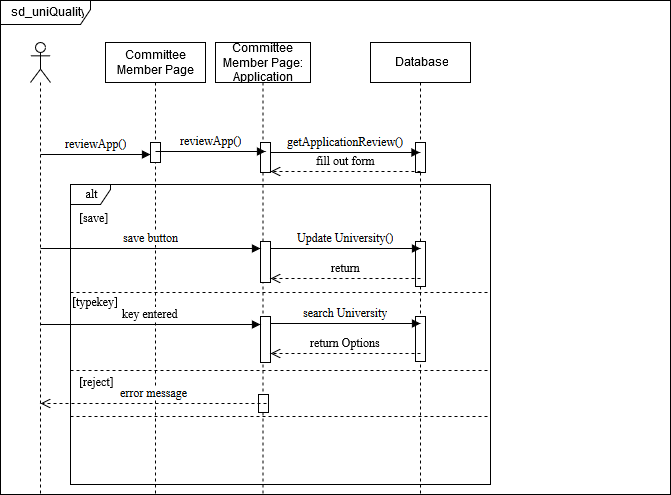
\includegraphics[width=.99\textwidth]{images/sd_uniQuality.png}
\end{center}
\caption{Sequence Diagram: Applying University Assessment}
\label{fig:sd_apply_uni}
\end{figure}


%%%%%%%%%%%%%%%%%%%%%%%%%%%%%%%%%%%%%%%%%%%

\clearpage
\newpage
\section{Human Interface Design}

\subsection{Overview of User Interface}

Refer to \url{http://www.cse.yorku.ca/~eddyv/gradapps/index.html}

\subsection{Screen Images}

\begin{figure}[!htb]
\begin{center}
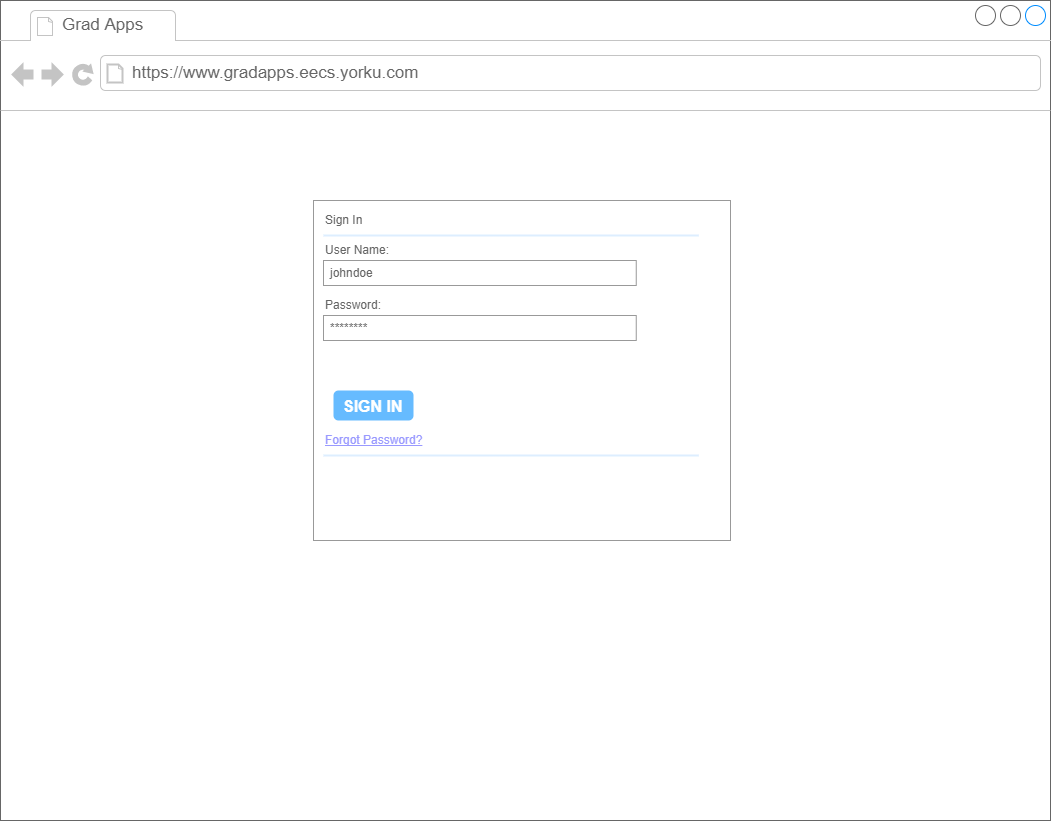
\includegraphics[width=.99\textwidth]{images/login_page.png}
\end{center}
\caption{Login Page View}
\label{fig:login_page_view}
\end{figure}

\begin{figure}[!htb]
\begin{center}
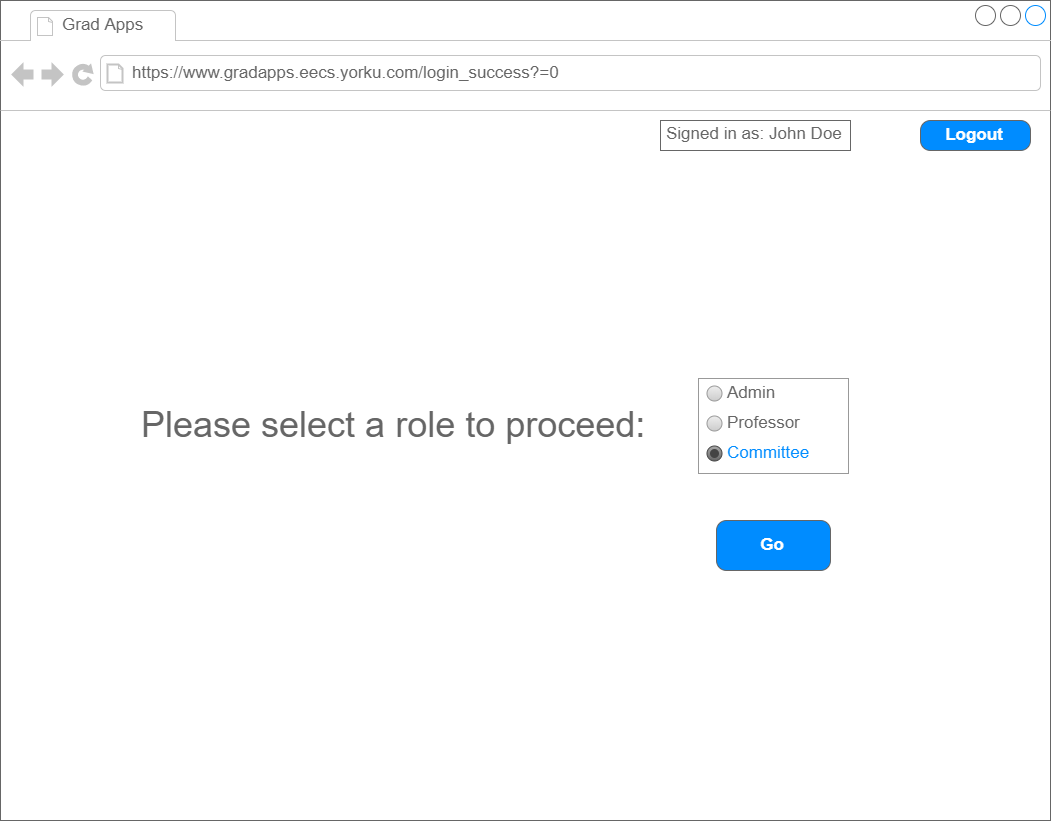
\includegraphics[width=.99\textwidth]{images/role_selection.png}
\end{center}
\caption{Role Selection View}
\label{fig:role_selection_view}
\end{figure}

\begin{figure}[!htb]
\begin{center}
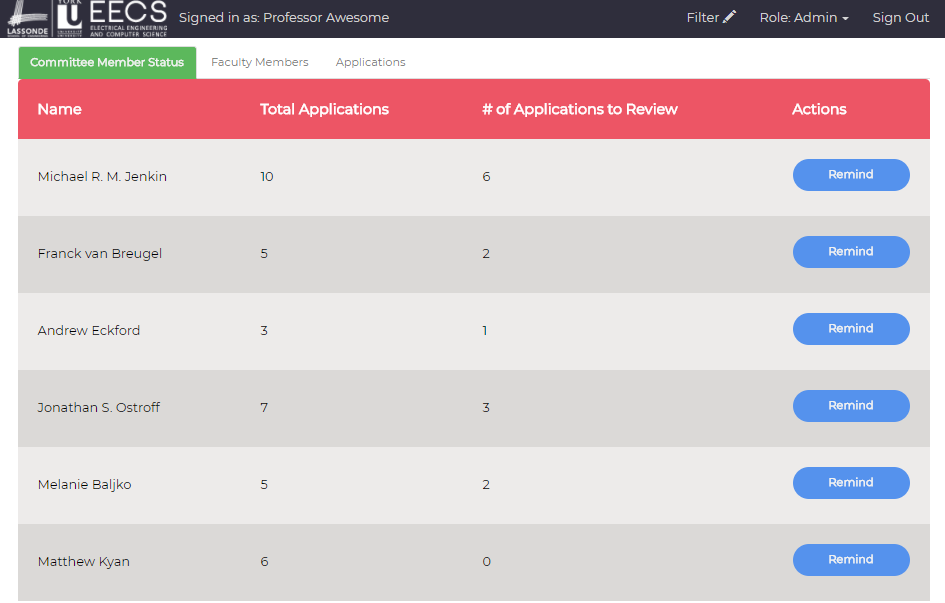
\includegraphics[width=.78\textwidth]{images/admin_view1.png}
\end{center}
\caption{Admin View - Committee Member Status}
\label{fig:admin_view1}
\end{figure}

\begin{figure}[!htb]
\begin{center}
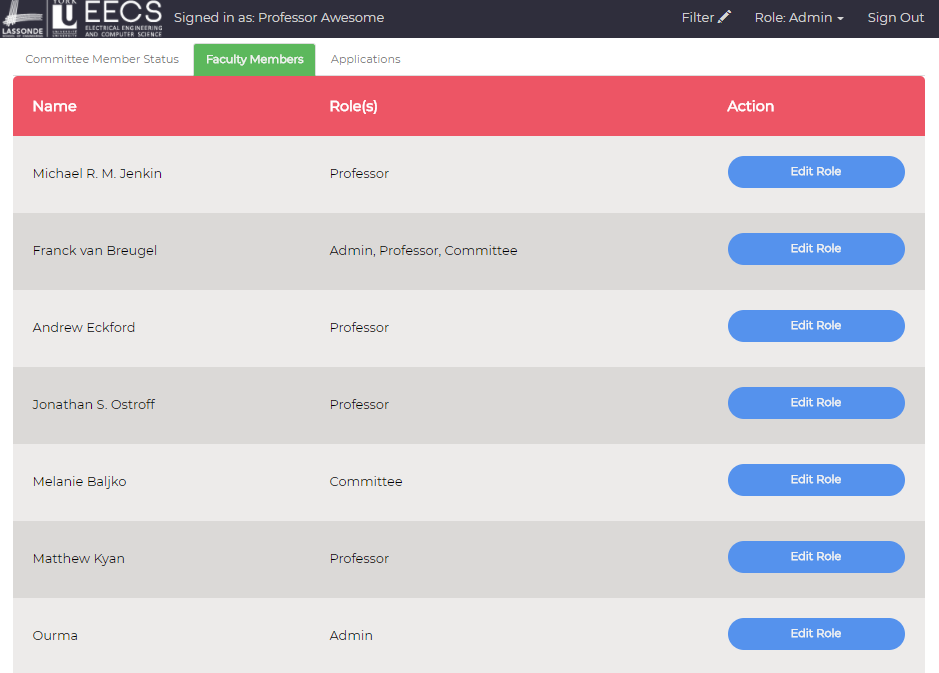
\includegraphics[width=.78\textwidth]{images/admin_view2.png}
\end{center}
\caption{Admin View - List Faculty Members}
\label{fig:admin_view2}
\end{figure}

\begin{figure}[!htb]
\begin{center}
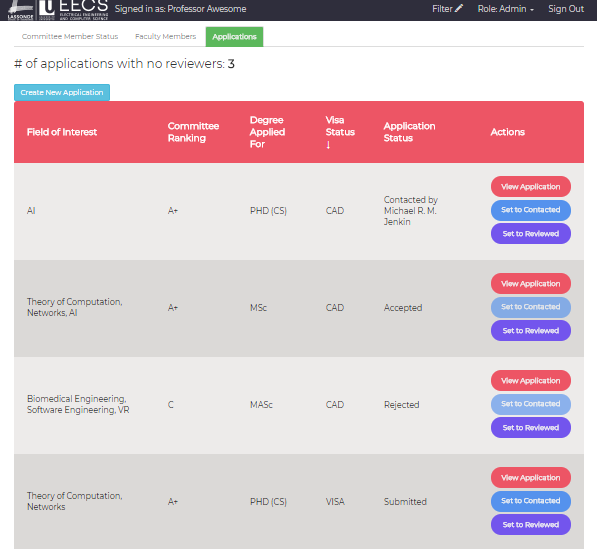
\includegraphics[width=.99\textwidth]{images/admin_prof_view.png}
\end{center}
\caption{Admin and Professor View - List of Student Applications}
\label{fig:admin_prof_view}
\end{figure}

\begin{figure}[!htb]
\begin{center}
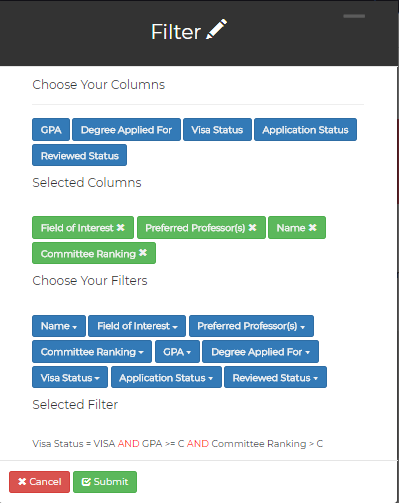
\includegraphics[width=.78\textwidth]{images/admin_prof_filter.png}
\end{center}
\caption{Filters available for the Admin and Professor role}
\label{fig:admin_prof_filter}
\end{figure}

\begin{figure}[!htb]
\begin{center}
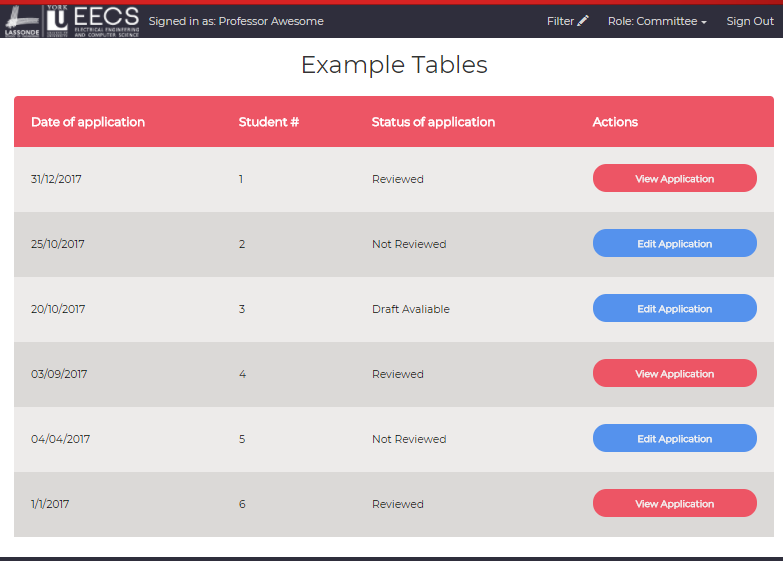
\includegraphics[width=.99\textwidth]{images/committee_view.png}
\end{center}
\caption{Committee View - List of review applications}
\label{fig:committee_view}
\end{figure}

\begin{figure}[!htb]
\begin{center}
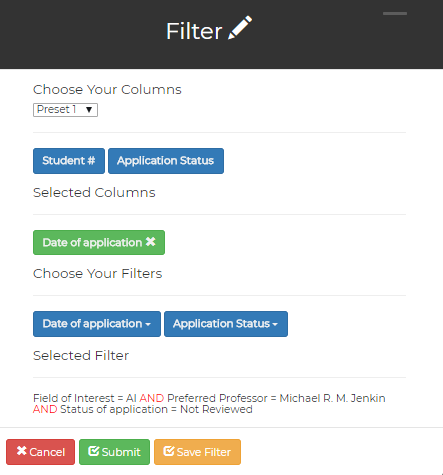
\includegraphics[width=.78\textwidth]{images/committee_filter.png}
\end{center}
\caption{Filters available for the Committee role}
\label{fig:committee_filter}
\end{figure}

\clearpage
\newpage
\subsection{Screen Objects and Actions}

The screenshots un the previous section from Figure \ref{fig:login_page_view} to \ref{fig:committee_filter} describes the flow of action an user may take for the System Under Description. The following describes each figure from the previous section.

\begin{itemize}
\item Figure \ref{fig:login_page_view} specifies the login view for the system. The login credentials shall be authenticated by Passport York. The user is expected to have a valid Passport York account and be part of the system database in order to gain access to the system.
\item Figure \ref{fig:role_selection_view} specifies the role selection view upon logging into the system. Once the user has been successfully authenticated into the system, the user needs to select a role to proceed further.
\item Figure \ref{fig:admin_view1} specifies the admin view of checking the committee member status. This view includes reminding a committee member who have been assigned a review and has not completed it yet.
\item Figure \ref{fig:admin_view2} specifies the admin view that lists all the members in the system. An admin can remove or change a role of a member. An admin can further add a new member into the system.
\item Figure \ref{fig:admin_prof_view} specifies the admin and professor view of all student applications in the system.
\item Figure \ref{fig:admin_prof_filter} specifies the admin and professor view of the filters available on student applications.
\item Figure \ref{fig:committee_view} specifies the committee member view of all applications needed for review in the system.
\item Figure \ref{fig:committee_filter} specifies the committee member view of the filters available on review applications.
\end{itemize}

%%%%%%%%%%%%%%%%%%%%%%%%%%%%%%%%%%%%%%%%%%%

\newpage
\section{Requirements Matrix}

The following table traces the primary R-descriptions from the Requirement Documentation which satisfies the design specified from Figure \ref{fig:login_page_view} to \ref{fig:committee_filter}. The R-descriptions are included in Appendix \ref{r-decs} to make it convenient for the reader.

\begin{table}[h]
\centering
\begin{tabular}{| c | c | c | c | c | c | c | c | c |}
	\cline{1-9}
	\textbf{REQ} & \textbf{Fig. \ref{fig:login_page_view}} & \textbf{Fig. \ref{fig:role_selection_view}} & \textbf{Fig. \ref{fig:admin_view1}} & \textbf{Fig. \ref{fig:admin_view2}} & \textbf{Fig. \ref{fig:admin_prof_view}} & \textbf{Fig. \ref{fig:admin_prof_filter}} & \textbf{Fig. \ref{fig:committee_view}} & \textbf{Fig. \ref{fig:committee_filter}}\\ \hline
	REQ1 & X & & & & & & & \\ \hline
	REQ2 & X & X & X & X & X & X & X & X \\ \hline
	REQ3 & X & X & X & X & X & X & X & X \\ \hline
	REQ4 & & X & X & X & X & X & X & X \\ \hline
	REQ5 & & X & & & & & & \\ \hline
	
	REQ6 & & X & X & X & X & X & X & X \\ \hline
	REQ7 & & & & X & & & & \\ \hline
	REQ8 & & & & X & & & & \\ \hline
	REQ9 & & & & X & & & & \\ \hline
	REQ10 & & & X & & & & & \\ \hline
	
	REQ11 & & & & & X & & & \\ \hline
	REQ12 & & & & & X & & & \\ \hline
	REQ13 & & & & & X & & & \\ \hline
	REQ14 & & & X & & & & & \\ \hline
	REQ15 & & & & & X & & & \\ \hline
	
	REQ16 & & & & & & & X & \\ \hline
	REQ17 & & & & & & & X & \\ \hline
	REQ18 & & & & & & & & X \\ \hline
	REQ19 & & & & & & & X & \\ \hline
	REQ20 & & & & & & & X & \\ \hline
	
	REQ21 & & & & & X & & & \\ \hline
	REQ22 & & & & & X & & & \\ \hline
	REQ23 & & & & & X & & & \\ \hline
	REQ24 & & & & & X & & & \\ \hline
	REQ25 & & & & & & X & & \\ \hline
	
	REQ26 & & & & & & & X & \\ \hline
	REQ27 & & & & X & & & & \\ \hline
	REQ28 & & & & & & & X & \\ \hline
\end{tabular}
\caption {Traceability Matrix for R-descriptions}
\label{tbl:trace_matrix}
\end{table}

%%%%%%%%%%%%%%%%%%%%%%%%%%%%%%%%%%%%%%%%%%%

\clearpage
\newpage
\section{Appendices}
\appendix

\section{E/R-Descriptions} \label{r-decs}

%%%%%%%%%%%%%%%%%%%%%%%%%%%%%%%%%E/R USE CASE 1%%%%%%%%%%%%%%%%%%%%%%%%%%%%%%%%
\subsection{Use Case 1 Authentication - E/R Descriptions}

\genenv{Each EECS graduate program member must have an unique username and password associated with their account via PPY.\\}{}
\label{E1}

\smallskip
\noindent \textbf{Rationale}: The login credentials will be handled through the Passport York. This is to simplify login uses and since this business system is under York University, PPY is the most secure option.

\edescription
{If the PPY is down for maintenance service, the system must not be accessible.\\}
{See Env. \ref{E1}}
\label{E2}

\smallskip
\noindent \textbf{Rationale}: Since the system heavily relies on PPY authentication, if PPY is scheduled down for maintenance, the system becomes inaccessible.

\rdescription
{A user shall be able to login to the system \emph{iff} they are a member of the EECS graduate program with a role assigned.\\}
{$user \in FM$}
\label{R1}

\smallskip
\noindent \textbf{Rationale}: A user shall be able to log into the system if they are a member of the EECS graduate program and have a role assigned to them. The login will be completed using Passport York Authentication (PPY).

\genreq
{A user shall be able to logout of the system \emph{iff} they are already logged in.\\}
{}
\label{R2}

\smallskip
\noindent \textbf{Rationale}: A user shall be able to log out of the system iff they are logged into the system through PPY.

\rdescription
{A user shall be not both logged in and logged out at the same time.\\}
{$(m\_loggedIn) \iff \neg (m\_loggedOut)$}
\label{R3}

\smallskip
\noindent \textbf{Rationale}: For security reasons a user cannot be both logged in and logged out at the same time. If a logged in account gets idle after 15 minutes, the user is automatically logged out (refer to Req. \ref{R4}).

\genreq
{A user shall be logged out of the system after a maximum of 15 minutes of idleness.\\}
{}
\label{R4}

\smallskip
\noindent \textbf{Rationale}: It is best practice to log out an idle user from a business critical system. This is to make sure the user does not stay logged on forever and to ensure liveness property on a user account.

\rdescription
{A user shall select a role from the list of roles they are assigned to once logged into the system.\\}
{List of all the roles are as specified in Section \ref{roles}.}
\label{R5}

\smallskip
\noindent \textbf{Rationale}: The roles available to the user upon logging into the system are the roles the user have been assigned to. A user cannot select a role that has not been assigned to them.

\rdescription
{A user shall be logged in with exactly \emph{one} role at any given time.\\}
{$\forall role1, role2 : (user.role = role1 \land user.role = role2) \implies (role1 = role2)$}
\label{R6}

\smallskip
\noindent \textbf{Rationale}: A logged in user cannot be logged in with two different roles. This is to avoid conflicting access control between two different roles.
%%%%%%%%%%%%%%%%%%%%%%%%%%%%%%%%%END E/R USE CASE 1%%%%%%%%%%%%%%%%%%%%%%%%%%%%%%

%%%%%%%%%%%%%%%%%%%%%%%%%%%%%%%%%E/R USE CASE 2%%%%%%%%%%%%%%%%%%%%%%%%%%%%%%%%
\subsection{Use Case 2 Add Student Application- E/R Descriptions}

\genenv
{The \emph{GPA} must manually compile an application received from the graduate office before sending it for review. \\}
{}
\label{E3}

\smallskip
\noindent \textbf{Rationale}: This is the manual work that needs to be done by the Graduate Program Assistant. The GPA has agreed it is in their best interest to manually compile all bits of information into one file before proceeding with the application.

\genreq
{An \emph{admin} shall be able to upload a student application to the portal.\\}
{}
\label{R7}

\smallskip
\noindent \textbf{Rationale}: Only an \emph{admin} user shall be able to assign applications for review to a graduate committee member. For simplicity, there is no maximum cap enforced for reviewing an application by a committee member.


%%%%%%%%%%%%%%%%%%%%%%%%%%%%%%%%%END E/R USE CASE 2%%%%%%%%%%%%%%%%%%%%%%%%%%%%%%

%%%%%%%%%%%%%%%%%%%%%%%%%%%%%%%%%E/R USE CASE 3%%%%%%%%%%%%%%%%%%%%%%%%%%%%%%%%
\subsection{Use Case 3 Add/Remove Members and Assign Roles- E/R Descriptions}

\genreq
{An \emph{admin} shall be able to add a new member to the list of EECS graduate program staff.\\}
{}
\label{R8}

\smallskip
\noindent \textbf{Rationale}: Only an \emph{admin} user shall be able to add a new member to the list of EECS graduate program staffs and assign one or more role(s) to them. In fact, an \emph{admin} shall be able to add a new member and assign them to the role of \emph{admin} as well.

\genreq
{An \emph{admin} shall be able to remove a member from the list of EECS graduate program staff except themselves.\\}
{}
\label{R9}

\smallskip
\noindent \textbf{Rationale}: Only an \emph{admin} user shall be able to remove an existing member from the list of EECS graduate program staffs. An \emph{admin} \textbf{cannot} remove themselves from the system.

\genreq
{An \emph{admin} shall be able to assign a new role to an existing faculty member with an old role except for themselves.\\}
{}
\label{R10}

\smallskip
\noindent \textbf{Rationale}: Only an \emph{admin} user shall be able to change existing roles of a registered user. An \emph{admin} \textbf{cannot} change their own role in the system.

\genreq
{An \emph{admin} shall be able to remove a role from an existing graduate program member with a at least one role assigned.\\}
{}
\label{R11}

\smallskip
\noindent \textbf{Rationale}: A \emph{admin} shall be able to remove a role assigned to an existing graduate member. This is to take away privileges on performing certain actions in the system. 
%%%%%%%%%%%%%%%%%%%%%%%%%%%%%%%%%END E/R USE CASE 3%%%%%%%%%%%%%%%%%%%%%%%%%%%%%%

%%%%%%%%%%%%%%%%%%%%%%%%%%%%%%%%%E/R USE CASE 4%%%%%%%%%%%%%%%%%%%%%%%%%%%%%%%%
\subsection{Use Case 4 Assign Application to Committee Member - E/R Descriptions}

\rdescription
{An \emph{admin} shall be able to assign applications for review to a graduate committee member.\\}
{The set $GC$ denotes the set of all graduate committee members which is a subset of all members in the system, $GC \subseteq FM$.}
\label{R12}

\smallskip
\noindent \textbf{Rationale}: Only an \emph{admin} user shall be able to assign applications for review to a graduate committee member. For simplicity, there is no maximum cap enforced for reviewing an application by a committee member.

\genreq
{A \emph{committee member} shall be notified when a batch of applications come in for review.\\}
{}
\label{R13}

\smallskip
\noindent \textbf{Rationale}: After an \emph{admin} sends out application(s) for review to a committee member, the \emph{committee member} gets an in app notification associated with their PPY.
%%%%%%%%%%%%%%%%%%%%%%%%%%%%%%%%%END E/R USE CASE 4%%%%%%%%%%%%%%%%%%%%%%%%%%%%%%

%%%%%%%%%%%%%%%%%%%%%%%%%%%%%%%%%E/R USE CASE 5%%%%%%%%%%%%%%%%%%%%%%%%%%%%%%%%
\subsection{Use Case 5 View/Filter Applications - E/R Descriptions}

\genreq
{An \emph{admin} shall be able to export the applications to CSV format.\\}
{}
\label{R14}

\smallskip
\noindent \textbf{Rationale}: Only an \emph{admin} user shall be able to download a CSV format of the applications and make changes to the file. Being able to import the changed CSV file is an optional requirement that may be implemented if time permits and all required deliverables have been achieved.

\genreq
{A \emph{committee member} shall be able to see the list of assigned application(s).\\}
{}
\label{R15}

\smallskip
\noindent \textbf{Rationale}: A \emph{committee member} shall be allowed to view a list of new (to be reviewed) and previously reviewed application(s). This will allow the committee members to have an organized view of the applications left to review and the applications that have been reviewed already.

\rdescription
{A \emph{committee member} shall be able to apply filtering only on selected attributes.\\}
{Refer to Table \ref{tbl:attr_reviewed}}
\label{R16}

\smallskip
\noindent \textbf{Rationale}: Allowing extra filtering on assigned application will cause favouritism of some student X while student Y will never get reviewed. Thus, it has been decided to only allow filtering on already reviewed application(s).

\rdescription
{An \emph{admin} shall be able to view a list of all student application(s).\\}
{refer to Req. \ref{R19}}
\label{R17}

\rdescription
{An \emph{professor} shall be able to view a list of student application(s) approved by an admin.\\}
{refer to Req. \ref{R19}}
\label{R18}

\smallskip
\noindent \textbf{Rationale}: An \emph{admin} and \emph{professor} shall be allowed to view a list of student application(s). The list of students shown can be narrowed/expanded using filters (refer to Req. \ref{R19}).

\genreq
{An \emph{admin} and \emph{professor} shall be able to filter on all student applications including personal attributes such as review status.\\}
{}
\label{R19}

\smallskip
\noindent \textbf{Rationale}: An \emph{admin} and a \emph{professor} shall be able to apply filters on a list of student applications. This is to allow narrow/expand searches of student on various attributes.
%%%%%%%%%%%%%%%%%%%%%%%%%%%%%%%%%END E/R USE CASE 5%%%%%%%%%%%%%%%%%%%%%%%%%%%%%%

%%%%%%%%%%%%%%%%%%%%%%%%%%%%%%%%%E/R USE CASE 6%%%%%%%%%%%%%%%%%%%%%%%%%%%%%%%%
\subsection{Use Case 6 Update Application- E/R Descriptions}

\genenv
{The \emph{GPA} must contact the institutions graduate admission office whenever there needs to be a form of communication. \\}
{}
\label{E4}

\smallskip
\noindent \textbf{Rationale}: The GPA can contact the institutions graduate admission office for further information on application if needed.

\genenv
{The \emph{GPA} must send the final decision of a student application to the institutions graduate admission office. \\}
{}
\label{E5}

\smallskip
\noindent \textbf{Rationale}: The GPA must send the final decision of an application to the institutions graduate admission office.

\rdescription
{An \emph{admin} shall be able to update all attributes of a student application.\\}
{refer to Table \ref{tbl:attr_uploaded}}
\label{R20}

\smallskip
\noindent \textbf{Rationale}: Only an \emph{admin} user shall be able to update all attributes of an application (refer to Table \ref{tbl:attr_uploaded}). This to allow updating secured information on the application that maybe confidential.

\rdescription
{The \emph{GPA} shall be notified when a \emph{professor} has requested a student for admission.\\}
{refer to Env. \ref{E5}}
\label{R21}

\smallskip
\noindent \textbf{Rationale}: The \emph{GPA} shall be notified when a \emph{professor} requests a student for admission. The graduate program assistant can then contact the graduate office with further information (refer to Env. \ref{E5}).

\genreq
{A \emph{professor} shall be able to review a student application.\\}
{}
\label{R22}

\smallskip
\noindent \textbf{Rationale}: A \emph{professor} shall be allowed to view a posted student application. Once an application has been viewed by the professor, it is automatically checked \textbf{Reviewed} and this status is only visible to the professor user who have viewed it. For all not reviewed applications, the \textbf{Reviewed Status} field is left empty.

\genreq
{A \emph{professor} shall be able to contact a student.\\}
{}
\label{R23}

\smallskip
\noindent \textbf{Rationale}: A \emph{professor} shall be allowed to contact a student once their application satisfies the professor's need. The contact shall need to be made through external email and the professor needs to update the application to \textbf{Contacted}. We leave this upto the user to use this feature correctly. The contacted status is visible to all graduate program members who have access to the portal (i.e all \emph{admins} and \emph{professors}).

\rdescription
{A \emph{professor} shall be able to request a student for admission.\\}
{refer to Req. \ref{R21} and Env. \ref{E5}}
\label{R24}

\smallskip
\noindent \textbf{Rationale}: A \emph{professor} shall be allowed to request a student for admission. Once the request has been sent in, the \emph{GPA} will receive a notification (refer to Req. \ref{R21}) and then can reach out the institutions graduate office with a request for admission (refer to Env. \ref{E5}).
%%%%%%%%%%%%%%%%%%%%%%%%%%%%%%%%%END E/R USE CASE 6%%%%%%%%%%%%%%%%%%%%%%%%%%%%%%

%%%%%%%%%%%%%%%%%%%%%%%%%%%%%%%%%E/R USE CASE 7%%%%%%%%%%%%%%%%%%%%%%%%%%%%%%%%
\subsection{Use Case 7 Review Student Application- E/R Descriptions}

\genreq
{The \emph{GPA} shall be notified when reviews for an application have been completed.\\}
{}
\label{R25}

\smallskip
\noindent \textbf{Rationale}: Only the \emph{GPA} shall be notified when the review has been completed. It shall be a 1-to-1 relation to avoid multiple levels of notification between users.

\genreq
{A \emph{committee member} shall be able to save ongoing reviews as a draft for future completion.\\}
{}
\label{R26}

\smallskip
\noindent \textbf{Rationale}: A \emph{committee member} shall be allowed to save ongoing reviews as a draft. A draft can be later resumed for completion. This gives the committee member an opportunity to not rush through the review.

\genreq
{A \emph{committee member} shall be able to view, use, add or modify a university assessment if it has already been provided.\\}
{}
\label{R27}

\smallskip
\noindent \textbf{Rationale}: A \emph{committee member} shall be allowed to view, use or modify a previous university assessment used in a review. This removes the work of typing in the same university assessment or even a modified assessment of a previously assessed university.

\rdescription
{A \emph{committee member} shall be able to submit a completed review to the \emph{GPA}.\\}
{Refer to Req. \ref{R25}}
\label{R28}

\smallskip
\noindent \textbf{Rationale}: A \emph{committee member} shall be able to submit a completed review to the \emph{GPA}. The \emph{GPA} can then upload the application to the portal for professors to access the application.
%%%%%%%%%%%%%%%%%%%%%%%%%%%%%%%%%END E/R USE CASE 7%%%%%%%%%%%%%%%%%%%%%%%%%%%%%%

\end{document}  